%---------- Inleiding ---------------------------------------------------------

\section{Introductie}%
\label{sec:introductie}
\noindent
De meestgekende nieuwsbronnen proberen al jaren objectief en feitelijk te blijven om informatie vanop eenzelfde standpunt en met een gelijkaardig boodschap over te brengen. 

\noindent
Binnen mijn toegepast onderzoek zal ik een toepassing maken die een kunstwerk zal genereren met behulp van één of meerdere deep learning modellen. Dit zou er voor zorgen dat het dagelijkse hoogtepunt geabstraheerd kan worden tot een unieke AI-gegenereerde kunstwerk.


%---------- Stand van zaken ---------------------------------------------------

\section{Literatuurstudie}%
\autocite{Salem2020}
\autocite{Lauri2019}



%---------- Methodologie ------------------------------------------------------
\section{Methodologie}%
\label{sec:methodologie}
\noindent
\textbf{Inleiding} \\
Het toegepast onderzoek begint 2 maart 2023 en zal beëindigd worden voor 28 mei 2023. \\

\noindent
\textbf{Fase 1: Realiseren van een scraper} \\
Om de data te bekomen van de verschillende soorten websites of social-media platformen zal er een web scraper worden gemaakt. Deze scraper zal ontwikkeld worden in python met behulp van een externe library \emph{BeautifulSoup}.

\noindent
Doordat de presentatie van de verschillende artikelen kunnen verschillen in taal en structuur, zal de scraper een algoritme implementeren die het mogelijk maakt om op een uniforme manier verschillende websites te scrapen. \\

\noindent
\textbf{Fase 2: Data verwerken en analyseren} \\
Tijdens de tweede fase zullen we onderzoeken op welke manier we de bekomen data uit voorgaande fase kunnen analyseren en sorteren. \\ \\
\noindent
Het zal belangrijk zijn om rekening te houden met de volgende vragen: 
\begin{itemize}
    \item Wat zijn de te extraheren kernzaken?
    \item Wat is het sentiment van de dag? 
    \item Welke topic komt het vaakst voor?
    \item Op basis van welke gegevens kunnen we de artikels sorteren? 
\end{itemize}

\noindent
Nadat er een gepaste methode wordt gevonden om dit te realiseren, zal deze ook geïmplementeerd worden. Op deze manier kunnen we steeds het belangrijkste artikel van de dag eruit halen. \\

\noindent
\textbf{Fase 3: Kunstwerk genereren} \\
Nu dat we weten uit de vorige fase wat het hoogtepunt van de dag was. Kunnen we hierop een kunstwerk laten genereren. \\
Hiervoor zal er gebruik gemaakt worden van een of meerdere deep learning modellen Dall-E en/of Stable Diffusion die de kerntekst van een artikel zal omvormen tot een foto. \\

\noindent
Één of beide technologieën zullen gebruikt worden. 



%---------- Verwachte resultaten ----------------------------------------------
\section{Verwacht resultaten}%
\label{sec:verwachte_resultaten}
\noindent
Een applicatie ontwerpen die dagelijks een kunstwerk kan genereren op basis van het hoogtepunt van de dag. \\

\noindent
Op 27 oktober, toen Marokko won van België tijdens de WK kon het hoogtepunt in België \emph{'Riots in Brussels after soccer game, painting'} geweest zijn. Hieronder vindt u enkele voorbeelden die gegenereerd zijn met behulp van Dall-E op basis van deze tekstinput.


\noindent
\begin{tabular}{llll}
   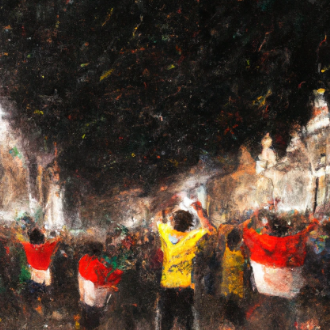
\includegraphics[width = 1.5in]{rellen_1.png} &
   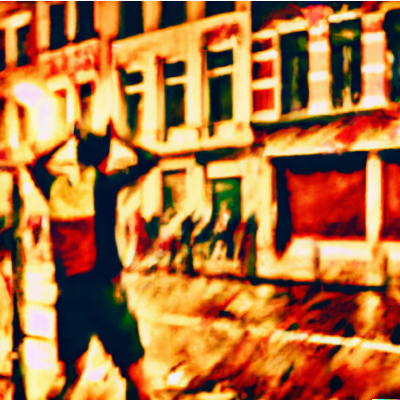
\includegraphics[width = 1.5in]{rellen_2.png} \\
   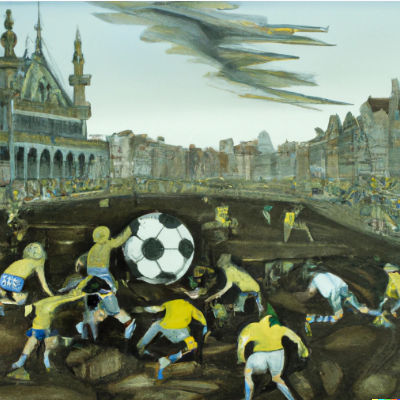
\includegraphics[width = 1.5in]{rellen_3.png} &
   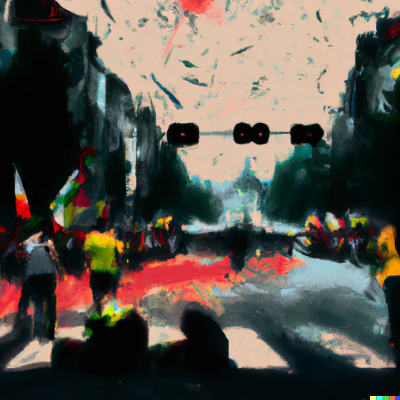
\includegraphics[width = 1.5in]{rellen_4.png}
\end{tabular}


